\newpage
\chapter{Index}
In this chapter an explanation of the index page (front page)  and the different thought and actions taken with it will be described.  
\section{Design Ideas}
The website is primarily to be used by a non-technical person at AU-Herning. The design has been kept clean to make it very intuitive how to navigate around. Periodically the energy system (and thereby also the website) is shown for high-schools students visiting the school, therefore the index page has been build up with mostly icons instead of text and a navigation bar which some of them might know from OS X (from Apple). The customer wanted the production shown as primitive things like: lightbulbs, refrigerators, money (possibly shown as number of SU payments), instead of technical terms like Joule, kW, kWh etc.
\section{The Design}

\begin{figure}[h!]
	\center
		\setlength\fboxsep{0pt}
		\setlength\fboxrule{1pt}
		\fbox{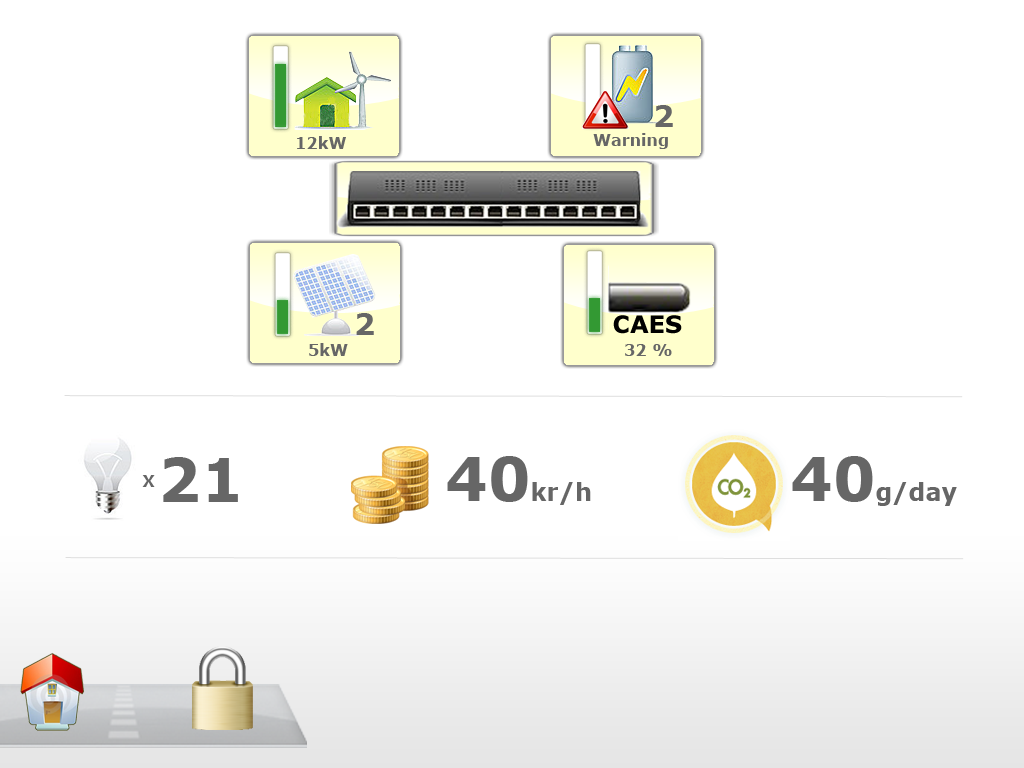
\includegraphics[width=0.6\textwidth]{images/index_design.png}}
   	\caption{First drawings of the index page.}
   	\label{fig:index_page_design}
\end{figure}
fdsa fdsa fdsa
\section{Code layout}
fdsa
\section{Code explanation}
fdsa
\subsection{CCS}
fdsa
\subsection{HTML}
fdsa
\newpage
HTML CODE
\begin{lstlisting}
   	<div id="bg">
    	<img src="pic/background.png" alt="background"/>
	</div>
	<div id="hub" class="boxbg">
    	<a href="hub.html"> <img src="pic/hub_big.png" alt="HUB Module"/> 		</a>
    </div>
    <div id="Mtopleft" class="boxbg">
    	<a href="wind.html"> <img src="pic/wind.png" alt="HUB Module"/> 		</a>
    </div>
    <div id="Mtopright" class="boxbg">
    	<a href="photo.html"> <img src="pic/photo.png" alt="HUB Module"/> 		</a>
    </div>
    <div id="Mbottomleft" class="boxbg">
    	<a href="caes.html"> <img src="pic/caes.png" alt="HUB Module"/> 		</a>
    </div>
    <div id="Mbottomright" class="boxbg">
    	<a href="battery.html"> <img src="pic/bat.png" alt="HUB Module"/> 		</a>
    </div>

\end{lstlisting}
CSS CODE
\begin{lstlisting}[language=CSS] 
/* DEVICES CONNECTED */
.boxbg {
	position:absolute;
	background-image:url(pic/ybg.png);
	background-repeat:repeat-x;
	height: 100px;
	width: 150px;
	border: 2px solid #999;	/* Put padding and round corners*/
	border-bottom-left-radius: 5px;
	border-bottom-right-radius: 5px;
	border-top-left-radius: 5px;
	border-top-right-radius: 5px;
}
\end{lstlisting}